\chapter{Slunce}

\section{Proč ho zkoumáme?}
Slunce je zdaleka nejbližší hvězda, můžeme ji tedy pozorovat s vysokým rozlišením prostorovým i časovým rozlišením a to jak dalekohledy z pozemských observatoří, tak umělými družicemi. Takovéhoto rozlišení nejsme u ostatních hvězd ani zdaleka schopni dosáhnout. Je to jediná hvězda, která nám umožňuje pozorovat jevy a struktury na jejím povrchu. Studování Slunce tedy velmi užitečné i pro zkoumání ostatních hvězd. Sluneční aktivita má vliv na takzvané vermírné počasí, kterým následně ovlivňuje i naši atmosféru.  Slunce je tvořeno převážně ionizovaným plynem – plazmatem, které vykazuje mnoho stejných vlastností, jako plazma uměle vytvořené na Zemi v tokamacích. Můžeme ho tedy využívat i jako laboratoř pro výzkum plazmatu~\cite{nasa_whysolar}.

\section{Stavba Slunce}
Zhruba vnitřní čtvrtinu poloměru Slunce tvoří jádro. Slunce získává svoji energii syntézou jader vodíku na hélium. Tato termonukleární reakce může probíhat pouze za velmi vysokých teplot a při vysokém tlaku – tyto podmínky jsou přítomné právě v jádru Slunce, kde je tlak zhruba $\unit[2.5\cdot10^{16}]{Pa}$ a teplota $\unit[1.5\cdot10^{7}]{K}$.

Na jádro navazuje zóna záření. Jak název napovídá, tak v této zóně probíhá přenos tepla především zářením. Střední volná dráha fotonu je v této oblasti přibližně $\unit[1]{mm}$~\cite{astro_hvezda}. Fotony, které jsou na začátku v rentgenovém spektru opouští zónu záření již jako viditelné světlo.

Kolem 0,72 poloměru (cca $\unit[490\,000]{km}$) je teplota plynu zhruba $\unit[2\,000\,000]{K}$ oproti $\unit[5\,000\,000]{K}$ na počátku zóny záření. To má za důsledek, že volné elektrony v plazmatu se opět spojují s jádry a vznikají atomy. Tím roste opacita plynu a stává se pro fotony neprůhledný a přenos energie zářením je již velmi neefektivní. Přenos energie v této oblasti probíhá prouděním, tedy konvekcí a tato oblast se nazývá konvektivní zóna.

Vzhledem k tomu, že Slunce je koule plynu, nelze přesně určit, kde je jeho povrch. Stanovujeme ho tedy pomocí takzvané optické hloubky $\tau$. Optická hloubka přibližně $\tau=1$ odpovídá tomu, že foton se na své cestě ze Slunce průměrně rozptýlí méně, než jedenkrát. Optická hloubka $\tau=1$ je tedy stanovena jako hloubka, kde přechází konvektivní vrstva ve fotosféru. Fotosféra nakonec volně přechází v chronosféru, pro níž je typická její velmi nízká hustota, cca $10^4$krát menší, než ve fotosféře.

Jednoduché schéma struktury Slunce je na obr. \ref{fig:stavba}.

\section{Magnetické pole Slunce}
Slunce má silné dipólové magnetické pole, podobně jako Země. Je zesilováno elektrickým proudem který v plazatu proudí kolem feromagnetického jádra. Proud je díky indukci zpomalován a zhruba každých 11 let mění svůj směr. Vzniká tak přírodní magnetohydrodynamický generátor.

Ionizovaný plyn díky vysoké permeabilitě unáší magnetické pole a dipólové pole je tedy deformováno diferenciální rotací (pozorujeme, že ionizovaný plyn na rovníku rotuje rychleji, než v okolí osy rotace) a chaotickými konvektivními pohyby.

Průměrná intenzita magnetického pole na povrchu slunce je přibližně $\unit[1]{G}$, díky výše zmíněným deformacím ovšem může dojít ke vzniku takzvaných aktivních oblastí, kde intenzita pole dosahuje až $\unit[4000]{G}$.

\begin{figure}[h!]
	\centering
	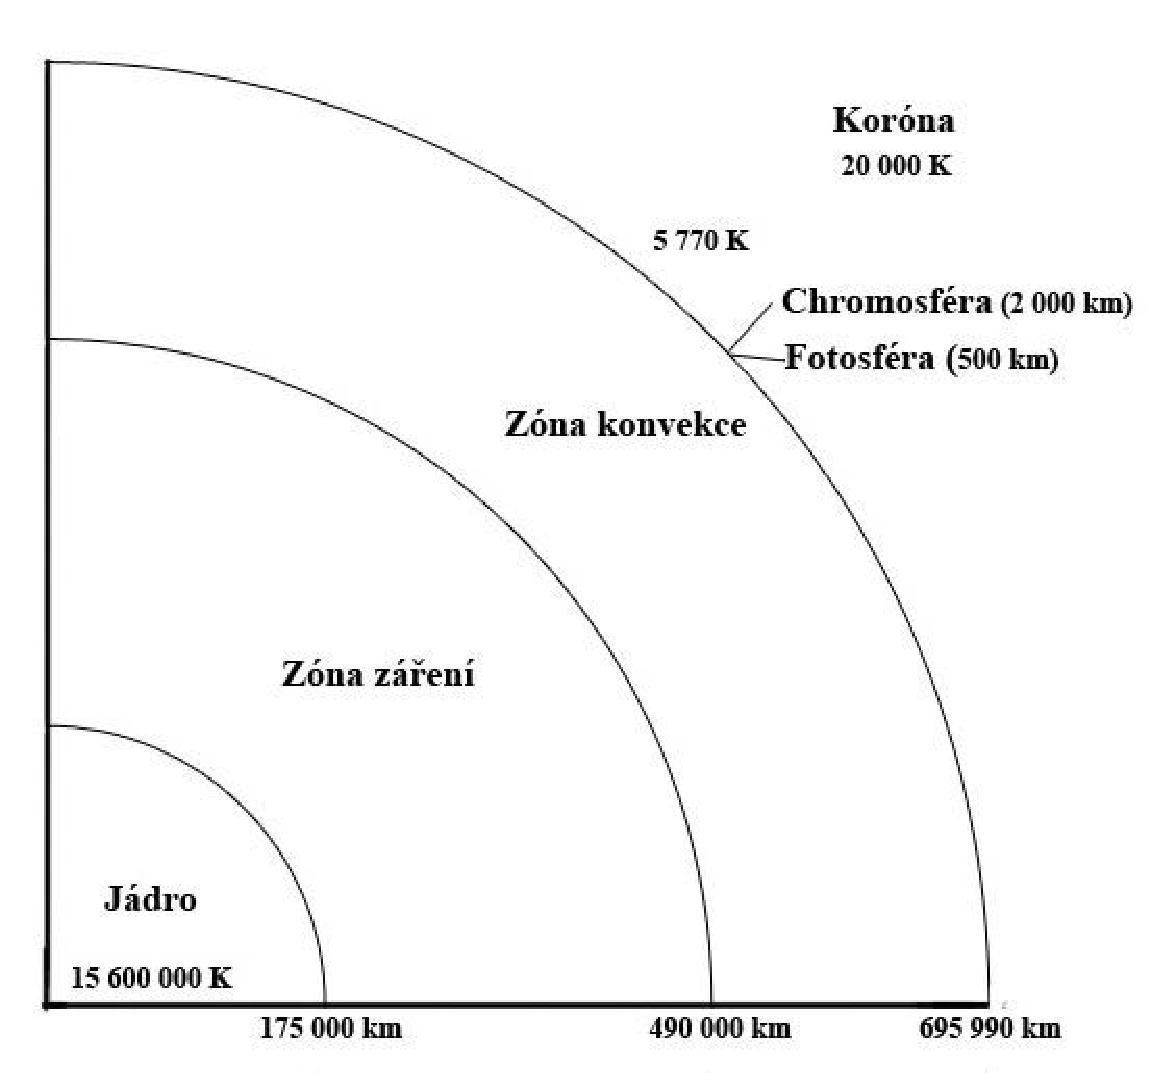
\includegraphics[scale=0.5]{../img/stavba_slunce.eps}
	\caption{Schéma jednotlivých vrstev Slunce - obrázek převzat z~\cite{astro_hvezda}}
	\label{fig:stavba}
\end{figure}